\documentclass[conference]{IEEEtran}
\usepackage{cite}
\usepackage{url}
\usepackage{booktabs}
\usepackage{amsmath}
\usepackage{xspace}
\usepackage{graphicx}
\usepackage{array}
% ponytail: BasicTeX here lacks Courier; on Overleaf this line can go
\renewcommand{\ttdefault}{cmtt}

% Every number below comes from make_numbers.py; regenerate, never hand-edit.
\newcommand{\nTriaged}{240}
\newcommand{\nAdmissible}{118}
\newcommand{\nCollectEmpty}{64}
\newcommand{\nStaticAttempted}{105}
\newcommand{\nStaticOk}{78}
\newcommand{\nPycgFail}{22}
\newcommand{\pctPycgFail}{21\%}
\newcommand{\nLayoutFail}{5}
\newcommand{\nPyrightOk}{100}
\newcommand{\nWithArtifacts}{100}
\newcommand{\medNodesOk}{181}
\newcommand{\medNodesFail}{935}
\newcommand{\minNodesFail}{16}
\newcommand{\minNodesFailRepo}{chevron}
\newcommand{\nFailTimeout}{15}
\newcommand{\nFailCrash}{4}
\newcommand{\nFailOom}{1}
\newcommand{\nFailMixed}{2}
\newcommand{\nNondet}{36}
\newcommand{\pctNondet}{46\%}
\newcommand{\medSpread}{1.0\%}
\newcommand{\nSpreadTen}{7}
\newcommand{\maxSpread}{65\%}
\newcommand{\maxSpreadRepo}{movingpandas}
\newcommand{\nondetLow}{9/22}
\newcommand{\nondetMed}{13/23}
\newcommand{\nondetHigh}{14/33}
\newcommand{\pycgMedSec}{0.7}
\newcommand{\pycgMaxSec}{582}
\newcommand{\jacMed}{0.65}
\newcommand{\jacQone}{0.56}
\newcommand{\jacQthree}{0.80}
\newcommand{\nJacBelowHalf}{16}
\newcommand{\nJacAboveEight}{19}
\newcommand{\pycgOnlyShare}{11\%}
\newcommand{\pyrightOnlyShare}{27\%}
\newcommand{\nEdgesUnion}{33{,}368}
\newcommand{\pending}{\textbf{[pending]}}
\newcommand{\nPoolMatched}{98{,}416}
\newcommand{\nQueued}{558}
\newcommand{\nRefSet}{14}
\newcommand{\nRoundOne}{20}
\newcommand{\roundOneStrata}{8 HIGH, 7 MED, 5 LOW}
\newcommand{\nRoundTwo}{20}
\newcommand{\shivycMakeIl}{29}
\newcommand{\shivycMakeAsm}{20}
\newcommand{\sampleClick}{140}
\newcommand{\sampleToolz}{60}
\newcommand{\pilotFusedFails}{8}
\newcommand{\nRuntimeRepos}{39}
\newcommand{\nRuntimeExcluded}{3}
\newcommand{\edgeUnionMed}{0.69}
\newcommand{\edgeUnionMissMed}{31\%}
\newcommand{\nLowRuntime}{6}
\newcommand{\edgeUnionMin}{0.03}
\newcommand{\edgeUnionMax}{1.00}
\newcommand{\edgePycgMed}{0.53}
\newcommand{\edgePyrightMed}{0.68}
\newcommand{\nPyrightBeatsPycg}{33}
\newcommand{\nObservedPairs}{10{,}882}
\newcommand{\edgeMedLow}{0.79 ($n{=}6$)}
\newcommand{\edgeMedMed}{0.65 ($n{=}13$)}
\newcommand{\edgeMedHigh}{0.69 ($n{=}20$)}
\newcommand{\itemPycgP}{0.87}
\newcommand{\itemPycgR}{0.51}
\newcommand{\itemPyrightP}{0.86}
\newcommand{\itemPyrightR}{0.69}
\newcommand{\itemUnionP}{0.85}
\newcommand{\itemUnionR}{0.70}
\newcommand{\itemNameP}{0.22}
\newcommand{\itemNameR}{1.00}
\newcommand{\nItems}{33{,}020}
\newcommand{\nRealItems}{7{,}282}
\newcommand{\nMissed}{2{,}163}
\newcommand{\pctMissShared}{69\%}
\newcommand{\pctMissReference}{38\%}
\newcommand{\pctUnnamed}{34\%}
\newcommand{\nUnnamed}{3{,}659}
\newcommand{\llmOneTwentyP}{0.60}
\newcommand{\llmOneTwentyR}{0.87}
\newcommand{\llmOneTwentyStaticP}{0.83}
\newcommand{\llmOneTwentyStaticR}{0.65}
\newcommand{\llmOneTwentyN}{5{,}616}
\newcommand{\llmTwentyP}{0.63}
\newcommand{\llmTwentyR}{0.83}
\newcommand{\llmTwentyStaticP}{0.83}
\newcommand{\llmTwentyStaticR}{0.65}
\newcommand{\llmTwentyN}{5{,}611}
\newcommand{\llmQwenP}{0.70}
\newcommand{\llmQwenR}{0.79}
\newcommand{\llmQwenStaticP}{0.83}
\newcommand{\llmQwenStaticR}{0.65}
\newcommand{\llmQwenN}{5{,}578}
\newcommand{\cvComb}{0.76 & 0.74 & 0.75}
\newcommand{\cvCombUnion}{0.83 & 0.65 & 0.73}
\newcommand{\cvMajority}{0.66 & 0.85 & 0.74}
\newcommand{\cvAnyLlm}{0.54 & 0.91 & 0.68}
\newcommand{\cvCombFone}{0.75}
\newcommand{\nCombItems}{5{,}573}
\newcommand{\nCombRepos}{39}
\newcommand{\loroComb}{0.80 & 0.73 & 0.76}
\newcommand{\rqThreeRows}{\texttt{ShivyC} & L & 1459 & 0.34 & 0.41 & 0.44 & \texttt{rejax} & H & 174 & 0.28 & 0.36 & 0.36 \\
\texttt{movingpandas} & L & 382 & 0.48 & 0.54 & 0.57 & \texttt{json-logging-python} & H & 86 & 0.29 & 0.41 & 0.41 \\
\texttt{rlm} & L & 142 & 0.35 & 0.79 & 0.79 & \texttt{tensortrade-ng} & H & 834 & 0.15 & 0.42 & 0.44 \\
\texttt{pr-agent} & L & 619 & 0.66 & 0.79 & 0.79 & \texttt{jsonapi-requests} & H & 153 & 0.48 & 0.50 & 0.52 \\
\texttt{TradingView-Screener} & L & 19 & 0.11 & 1.00 & 1.00 & \texttt{redbeat} & H & 63 & 0.59 & 0.59 & 0.60 \\
\texttt{throttled} & L & 13 & 1.00 & 1.00 & 1.00 & \texttt{pyrlp} & H & 120 & 0.53 & 0.64 & 0.65 \\
\texttt{pysui} & M & 1393 & 0.24 & 0.27 & 0.27 & \texttt{django-ses} & H & 3 & 0.67 & 0.67 & 0.67 \\
\texttt{sqllineage} & M & 761 & 0.29 & 0.44 & 0.45 & \texttt{aws-dynamodb-encryption} & H & 74 & 0.58 & 0.61 & 0.68 \\
\texttt{sec-edgar} & M & 123 & 0.27 & 0.46 & 0.49 & \texttt{apiflask} & H & 142 & 0.47 & 0.68 & 0.69 \\
\texttt{pykwalify} & M & 192 & 0.43 & 0.51 & 0.53 & \texttt{click} & H & 704 & 0.46 & 0.68 & 0.69 \\
\texttt{PyFunceble} & M & 1045 & 0.25 & 0.47 & 0.54 & \texttt{compressed-tensors} & H & 413 & 0.50 & 0.68 & 0.70 \\
\texttt{confluence-md-exporter} & M & 206 & 0.51 & 0.58 & 0.58 & \texttt{deepblast} & H & 29 & 0.69 & 0.76 & 0.76 \\
\texttt{term-image} & M & 336 & 0.43 & 0.62 & 0.65 & \texttt{marshmallow-sqlalchemy} & H & 38 & 0.68 & 0.76 & 0.76 \\
\texttt{toolz} & M & 121 & 0.56 & 0.61 & 0.67 & \texttt{scrapyrt} & H & 25 & 0.72 & 0.80 & 0.80 \\
\texttt{fastapi-injectable} & M & 46 & 0.70 & 0.83 & 0.83 & \texttt{xacro} & H & 140 & 0.84 & 0.84 & 0.85 \\
\texttt{all-repos} & M & 221 & 0.80 & 0.82 & 0.83 & \texttt{geocube} & H & 45 & 0.64 & 0.87 & 0.87 \\
\texttt{mcp-seq-thinking} & M & 36 & 0.72 & 0.89 & 0.89 & \texttt{autoray} & H & 50 & 0.86 & 0.74 & 0.88 \\
\texttt{bedrock-agentcore-sdk} & M & 356 & 0.68 & 0.92 & 0.92 & \texttt{neutronclient} & H & 47 & 0.91 & 0.94 & 0.94 \\
\texttt{creosote} & M & 63 & 0.92 & 0.92 & 0.92 & \texttt{puncover} & H & 22 & 0.68 & 0.95 & 0.95 \\
\texttt{lazy-object-proxy} & H & 187 & 0.02 & 0.03 & 0.03 &  & & & & &  \\}
\newcommand{\rqFourKindRows}{call, unique name & 801 & 0.95 / 0.84 & 0.95 / 0.80 & 0.98 / 0.81 & 0.98 / 0.82 \\
call, shared name & 1798 & 0.44 / 0.74 & 0.67 / 0.60 & 0.75 / 0.57 & 0.52 / 0.71 \\
class name & 417 & 0.92 / 0.96 & 0.90 / 0.64 & 0.90 / 0.58 & 0.89 / 0.85 \\
reference, unique name & 1139 & 0.05 / 0.88 & 0.86 / 0.35 & 0.86 / 0.32 & 0.84 / 0.42 \\
reference, shared name & 1456 & 0.00 / 0.00 & 0.76 / 0.43 & 0.83 / 0.38 & 0.74 / 0.42 \\}
\newcommand{\kindSharedStaticR}{0.44}
\newcommand{\kindSharedLlmR}{0.52--0.75}
\newcommand{\kindRefStaticR}{0.05}
\newcommand{\kindRefLlmR}{0.74--0.86}
\newcommand{\kindRefLlmP}{0.32--0.43}
\newcommand{\llmBeatsMin}{15}
\newcommand{\llmBeatsMax}{18}
\newcommand{\llmReposN}{39}
\newcommand{\covSpearman}{-0.33}
\newcommand{\testsSpearman}{-0.23}
\newcommand{\covMed}{67\%}
\newcommand{\covMin}{24\%}
\newcommand{\covMax}{98\%}
\newcommand{\nRetrace}{37}
\newcommand{\retraceJacMin}{0.99}
\newcommand{\retraceJacMed}{1.00}
\newcommand{\compMissedR}{0.46--0.70}
\newcommand{\compFoundR}{0.94--0.97}
\newcommand{\nCompMissed}{483}
\newcommand{\ciOneTwentyPrec}{[0.51, 0.67]}
\newcommand{\ciOneTwentyRec}{[0.78, 0.95]}
\newcommand{\ciOneTwentyFone}{[0.64, 0.77]}
\newcommand{\ciTwentyPrec}{[0.53, 0.70]}
\newcommand{\ciTwentyRec}{[0.75, 0.90]}
\newcommand{\ciTwentyFone}{[0.65, 0.77]}
\newcommand{\ciQwenPrec}{[0.63, 0.76]}
\newcommand{\ciQwenRec}{[0.71, 0.87]}
\newcommand{\ciQwenFone}{[0.70, 0.78]}
\newcommand{\ciStaticPrec}{[0.75, 0.88]}
\newcommand{\ciStaticRec}{[0.55, 0.74]}
\newcommand{\ciStaticFone}{[0.66, 0.78]}
\newcommand{\staticPrecUniqueCall}{0.88}
\newcommand{\staticPrecSharedCall}{0.73}
\newcommand{\staticRecallSharedCall}{0.44}
\newcommand{\pycgRecallCtor}{0.49}
\newcommand{\pyrightRecallCtor}{0.95}
\newcommand{\loroRows}{PyCG & 0.84 & 0.49 & 0.62 \\
Pyright & 0.83 & 0.64 & 0.73 \\
PyCG $\cup$ Pyright & 0.83 & 0.65 & 0.73 \\
majority of the three LLMs & 0.66 & 0.85 & 0.74 \\
static $\cup$ any LLM & 0.54 & 0.91 & 0.68 \\
learned combiner & 0.80 & 0.73 & 0.76 \\}
\newcommand{\loroCombFone}{0.76}
\newcommand{\loroUnionFone}{0.73}
\newcommand{\loroMajorityFone}{0.74}
\newcommand{\loroCombP}{0.80}
\newcommand{\loroCombR}{0.73}
\newcommand{\loroUnionP}{0.83}
\newcommand{\loroUnionR}{0.65}
\newcommand{\nLoroBeats}{20}
\newcommand{\nLoroWorse}{9}
\newcommand{\nLoroRepos}{39}
\newcommand{\densitySpearman}{-0.23}
\newcommand{\thrLowMed}{4.0}
\newcommand{\thrMedHigh}{10.0}
\newcommand{\ciEdgeUnionMed}{[0.60, 0.79]}
\newcommand{\covSpearmanExact}{-0.325}
\newcommand{\covSpearmanP}{0.046}
\newcommand{\covSpearmanCI}{[-0.58, 0.00]}
\newcommand{\testsSpearmanExact}{-0.231}
\newcommand{\testsSpearmanP}{0.158}
\newcommand{\testsSpearmanCI}{[-0.54, 0.13]}
\newcommand{\densitySpearmanExact}{-0.230}
\newcommand{\densitySpearmanP}{0.156}
\newcommand{\densitySpearmanCI}{[-0.53, 0.11]}
\newcommand{\pyrMinusPycgMed}{0.08}
\newcommand{\ciPyrMinusPycgMed}{[0.06, 0.15]}
\newcommand{\pyrPycgWilcoxonP}{<0.001}
\newcommand{\nPyrPycgTies}{5}
\newcommand{\nPyrPycgReversals}{1}
\newcommand{\nPycgRun}{100}
\newcommand{\pctPycgFailRun}{22\%}
\newcommand{\nPycgAnySeedFail}{24}
\newcommand{\pctPycgSeedRunsFailed}{23\%}
\newcommand{\poolRecallPycg}{0.39}
\newcommand{\poolRecallPyright}{0.52}
\newcommand{\poolRecallUnion}{0.54}
\newcommand{\nMissAll}{4{,}953}
\newcommand{\missUnnamedOther}{34\%}
\newcommand{\medMissUnnamedOther}{32\%}
\newcommand{\missUnnamedDunder}{22\%}
\newcommand{\medMissUnnamedDunder}{13\%}
\newcommand{\missCallShared}{23\%}
\newcommand{\medMissCallShared}{6\%}
\newcommand{\missCallUnique}{3\%}
\newcommand{\medMissCallUnique}{0\%}
\newcommand{\missRefShared}{6\%}
\newcommand{\medMissRefShared}{0\%}
\newcommand{\missRefUnique}{10\%}
\newcommand{\medMissRefUnique}{11\%}
\newcommand{\missCtor}{1\%}
\newcommand{\medMissCtor}{0\%}
\newcommand{\missDecompRows}{unnamed: library or callback & 1{,}704 & 34\% \\
call, shared name & 1{,}157 & 23\% \\
unnamed: special method & 1{,}103 & 22\% \\
reference, unique name & 499 & 10\% \\
reference, shared name & 321 & 6\% \\
call, unique name & 136 & 3\% \\
class name & 33 & 1\% \\}
\newcommand{\missDecompRowsMed}{unnamed: library or callback & 1{,}704 & 34\% & 32\% \\
call, shared name & 1{,}157 & 23\% & 6\% \\
unnamed: special method & 1{,}103 & 22\% & 13\% \\
reference, unique name & 499 & 10\% & 11\% \\
reference, shared name & 321 & 6\% & 0\% \\
call, unique name & 136 & 3\% & 0\% \\
class name & 33 & 1\% & 0\% \\}
\newcommand{\medMissUnnamedAll}{57\%}
\newcommand{\missSharedAll}{30\%}
\newcommand{\missUnnamedAll}{57\%}
\newcommand{\missReferenceAll}{17\%}
\newcommand{\nUnnamedFound}{852}
\newcommand{\pctUnnamedFound}{23\%}
\newcommand{\nSelfCallItems}{59}
\newcommand{\nReflectCalls}{213}
\newcommand{\pctReflectCalls}{2\%}
\newcommand{\reflectMissRate}{0.50}
\newcommand{\plainMissRate}{0.45}
\newcommand{\pctMissReflective}{2\%}
\newcommand{\nSampleCallers}{940}
\newcommand{\nSampleStaticOnly}{53}
\newcommand{\sampleBaseRate}{24\%}
\newcommand{\woStaticP}{0.88}
\newcommand{\woStaticR}{0.64}
\newcommand{\woLlmR}{0.78--0.87}
\newcommand{\woLlmP}{0.61--0.73}
\newcommand{\loroDiffUnion}{0.04}
\newcommand{\ciLoroDiffUnion}{[0.00, 0.07]}
\newcommand{\loroDiffPyright}{0.04}
\newcommand{\ciLoroDiffPyright}{[0.00, 0.07]}
\newcommand{\loroCheckFone}{0.76}
\newcommand{\loroNorefCombFone}{0.75}
\newcommand{\loroNorefUnionFone}{0.70}
\newcommand{\ciLoroNorefDiffUnion}{[0.01, 0.09]}
\newcommand{\nLoroNorefRepos}{37}
\newcommand{\pctUnnamedDunder}{38\%}
\newcommand{\unnamedTopRepo}{pysui}
\newcommand{\pctUnnamedTopOfRest}{52\%}
\newcommand{\nTenSeed}{78}
\newcommand{\nSwept}{37}
\newcommand{\nSweptVaries}{8}
\newcommand{\sweepMaxPts}{10}
\newcommand{\sweepMaxDelta}{0.10}
\newcommand{\sweepMedDelta}{0.00}
\newcommand{\sweepWorstRepo}{term-image}
\newcommand{\sweepWorstLo}{0.34}
\newcommand{\sweepWorstHi}{0.43}
\newcommand{\sweepMedPts}{0.0}
\newcommand{\sweepMaxGraphs}{7}
\newcommand{\sweepUnionMaxPts}{2}
\newcommand{\sweepUnionMaxDelta}{0.02}
\newcommand{\nMixedTermination}{4}
\newcommand{\mixedTerminationRepo}{CorridorKey}
\newcommand{\nSetSwept}{77}
\newcommand{\nSetNondet}{21}
\newcommand{\setJacMin}{0.40}
\newcommand{\setJacMinRepo}{python-lazy-object-proxy}
\newcommand{\nVaryObserved}{8}
\newcommand{\nRawOnly}{16}
\newcommand{\nHiddenByCount}{2}
\newcommand{\nCountNondetSwept}{35}
\newcommand{\chevPasses}{100}
\newcommand{\chevDefsFirst}{177}
\newcommand{\chevDefsLast}{1420}
\newcommand{\chevGrowth}{12}
\newcommand{\chevRepeats}{0}
\newcommand{\muscNamesFirst}{555}
\newcommand{\muscNamesLast}{18{,}387}
\newcommand{\muscPasses}{4}
\newcommand{\muscLastPassMin}{22}
\newcommand{\setJacMed}{0.98}
\newcommand{\setJacQone}{0.94}
\newcommand{\setJacQthree}{1.00}
\newcommand{\nSetJacBelowNine}{3}
\newcommand{\setSweptMissingRepo}{deepblast}
\newcommand{\nRepeatSeedRuns}{156}
\newcommand{\nRepeatSeedAgree}{156}
\newcommand{\nRepeatEdgeIdentical}{40}
\newcommand{\nRepeatEdgeDiffer}{0}
\newcommand{\nRepeatNondetRepos}{36}
\newcommand{\nRepeatNondetRuns}{70}
\newcommand{\nRepeatNondetEqual}{70}
\newcommand{\nBigRepos}{36}
\newcommand{\nSmallRepos}{3}
\newcommand{\bigMedPycg}{0.52}
\newcommand{\bigMedPyright}{0.66}
\newcommand{\bigMedUnion}{0.68}
\newcommand{\bigPyrightWins}{32}
\newcommand{\bigDensitySpearman}{-0.09}
\newcommand{\bigDensitySpearmanP}{0.604}
\newcommand{\kwStrataH}{1.06}
\newcommand{\kwStrataP}{0.590}
\newcommand{\bestLlm}{qwen3.8-27b}
\newcommand{\loroRowsCI}{PyCG & 0.84 & 0.49 & 0.62 & [0.08, 0.19] \\
Pyright & 0.83 & 0.64 & 0.73 & [0.00, 0.07] \\
PyCG $\cup$ Pyright & 0.83 & 0.65 & 0.73 & [0.00, 0.07] \\
gpt-oss-20b & 0.63 & 0.83 & 0.71 & [0.00, 0.11] \\
gpt-oss-120b & 0.60 & 0.87 & 0.71 & [0.01, 0.11] \\
qwen3.8-27b & 0.70 & 0.79 & 0.74 & [$-$0.02, 0.06] \\
majority of the three LLMs & 0.66 & 0.85 & 0.74 & [$-$0.02, 0.08] \\
Pyright $\cup$ qwen3.8-27b & 0.70 & 0.81 & 0.75 & [$-$0.03, 0.06] \\
static $\cup$ any LLM & 0.54 & 0.91 & 0.68 & [0.03, 0.16] \\
learned combiner & 0.80 & 0.73 & 0.76 &  \\}
\newcommand{\nMapRepos}{37}
\newcommand{\mapPoolStrict}{0.38}
\newcommand{\mapMedStrict}{0.53}
\newcommand{\mapPoolLenient}{0.42}
\newcommand{\mapMedLenient}{0.58}
\newcommand{\mapPoolPyright}{0.51}
\newcommand{\mapMedPyright}{0.68}
\newcommand{\mapPoolUnionLenient}{0.54}
\newcommand{\mapMedUnionLenient}{0.69}
\newcommand{\mapPoolUnionStrict}{0.53}
\newcommand{\mapMedUnionStrict}{0.69}
\newcommand{\mapPyrWinsStrict}{31}
\newcommand{\mapPyrWinsLenient}{30}
\newcommand{\mapCtorStrict}{0.50}
\newcommand{\mapCtorLenient}{0.92}
\newcommand{\mapCtorPyright}{0.95}
\newcommand{\nMapAudited}{1{,}492}
\newcommand{\nMapLoss}{355}
\newcommand{\pctMapLoss}{24\%}
\newcommand{\pctMapLossSample}{30\%}
\newcommand{\mapUnionPoolDelta}{0.002}

\providecommand{\nRuntimeRepos}{\pending}
\providecommand{\rqThreeAbstract}{\pending}
\providecommand{\rqFourAbstract}{\pending}
\providecommand{\rqFourSampleNote}{}
\providecommand{\rqFourCvNote}{\pending}
\providecommand{\rqThreeBody}{\pending}
\providecommand{\rqFourBody}{\pending}
\providecommand{\rqDiscussionLlm}{\pending}
\providecommand{\rqConclusion}{\pending}
\IfFileExists{rq34.tex}{% RQ3/RQ4 prose. Numbers are macros from numbers.tex (make_numbers.py <- study1-results/rq34.json).
\providecommand{\cvComb}{--- & --- & ---}
\providecommand{\cvCombUnion}{--- & --- & ---}
\providecommand{\cvMajority}{--- & --- & ---}
\providecommand{\cvAnyLlm}{--- & --- & ---}
\providecommand{\loroComb}{--- & --- & ---}
\providecommand{\nCombItems}{\pending}
\providecommand{\nCombRepos}{\pending}

\renewcommand{\rqThreeAbstract}{the union of both analysers contains a median of \edgeUnionMed{} of
the calls observed (range \edgeUnionMin--\edgeUnionMax), and \pctMissShared{} of the calls it misses
go through a method name shared by several functions.}

\renewcommand{\rqFourAbstract}{raise recall on hard items from \llmTwentyStaticR{} to \llmQwenR--\llmOneTwentyR{} but lower
precision from \llmTwentyStaticP{} to \llmOneTwentyP--\llmQwenP; they find calls static analysis misses and claim calls that never happen, and a learned
combination of both does not generalise to unseen projects.}

\renewcommand{\rqFourSampleNote}{Each corpus repository contributes at most 25 sampled callers;
\texttt{click} and \texttt{toolz}, traced earlier, contribute 140 and 60.}

\renewcommand{\rqFourCvNote}{once with folds grouped by caller function, so that no function's
items are scored by a model trained on them, and once leaving out one whole repository at a time.}

\renewcommand{\rqThreeBody}{%
We traced the test suites of 20 of the sampled repositories, stratified by dynamism, plus
\texttt{click} and \texttt{toolz} from the scorer's reference set. Two could not be measured:
\texttt{kolla-ansible}'s tests never import its own package, and \texttt{wsgidav}'s suite produced
no countable test results under the harness. Across the remaining \nRuntimeRepos{} repositories the
tests exercised \nObservedPairs{} distinct calls between functions and methods of the packages.
Table~\ref{tab:recall} lists each repository.

\begin{table}[t]
\caption{Static recall against calls observed under each test suite.
Pairs: distinct caller$\to$callee calls observed. Edge columns: share of them in each static
graph. Item: recall of the union on call-resolution items.}\label{tab:recall}
\centering\footnotesize
\setlength{\tabcolsep}{4pt}
\begin{tabular}{llrrrrr}
\toprule
Repository & S & Pairs & PyCG & Pyright & Union & Item \\
\midrule
\rqThreeRows
\midrule
\multicolumn{3}{l}{Median over repositories} & \edgePycgMed & \edgePyrightMed & \edgeUnionMed & \\
\bottomrule
\end{tabular}
\end{table}

\textbf{How much is missing.} The union of both static graphs contains a median of
\edgeUnionMed{} of the observed calls per repository, from \edgeUnionMin{} to \edgeUnionMax{}.
Pyright alone reaches \edgePyrightMed{} and PyCG \edgePycgMed{}; Pyright finds more of the
observed calls in \nPyrightBeatsPycg{} of \nRuntimeRepos{} repositories, so in this corpus the
type checker is the stronger call-graph source. Pooled over \nItems{} call-resolution items
(\nRealItems{} of them observed calls), the union has precision \itemUnionP{} and recall
\itemUnionR{} (PyCG \itemPycgP/\itemPycgR, Pyright \itemPyrightP/\itemPyrightR). Plain name
matching, which treats every name on an executed line as a call, has precision \itemNameP{}: most
names in code that ran are not calls that happened.

\textbf{Where it misses.} Of the \nMissed{} observed calls the union misses, \pctMissShared{} go
to a method whose name is shared by several functions in the package, that is, dispatch over a
class hierarchy or over unrelated classes with a common method name, and \pctMissReference{} are
names written without call syntax, such as property reads and functions passed as values. The
worst repository illustrates the first pattern: \texttt{ShivyC}, a C compiler, defines
\texttt{make\_il} on 29 syntax-tree classes and \texttt{make\_asm} on 20, and the static union
holds fewer than half of its observed calls. A further \nUnnamed{} observed calls
(\pctUnnamed{} of all calls) reach a function never named in the calling function, typically a
callback stored elsewhere; no resolver that reads the caller's code can recover these.

\textbf{Dynamism did not predict recall.} The corpus was stratified by an AST score of reflective
and dynamic constructs, yet median union recall is similar across strata: \edgeMedLow{} for LOW, \edgeMedMed{} for MED
and \edgeMedHigh{} for HIGH. The constructs such scores count, reflection and dynamic imports, are
not where static analysers lose most calls on real code; ordinary polymorphic dispatch is.}

\renewcommand{\rqFourBody}{%
Table~\ref{tab:llm} compares the LLMs with the static union on the sampled callers, which are
enriched for hard items. Every LLM finds more of the observed calls than static analysis does:
recall rises from \llmTwentyStaticR{} for the static union on the same items to \llmTwentyR{} for gpt-oss-20b, \llmOneTwentyR{} for gpt-oss-120b and \llmQwenR{} for qwen3.8-27b.
Precision falls from \llmTwentyStaticP{} to between \llmOneTwentyP{} and \llmQwenP: the models claim calls
that never happen. The larger gpt-oss model has the highest recall and the lowest precision.
On real code, then, the micro-benchmark finding that PyCG outperforms LLMs~\cite{venkatesh2025llmcg}
holds for precision but reverses for recall.

\begin{table}[t]
\caption{Call resolution on the LLM sample. Top: each resolver on the items it answered.
Bottom: the items every LLM answered, scored out-of-fold.}\label{tab:llm}
\centering\footnotesize
\begin{tabular}{lrrr}
\toprule
Resolver (items) & Precision & Recall & \\
\midrule
gpt-oss-20b (\llmTwentyN) & \llmTwentyP & \llmTwentyR & \\
gpt-oss-120b (\llmOneTwentyN) & \llmOneTwentyP & \llmOneTwentyR & \\
qwen3.8-27b (\llmQwenN) & \llmQwenP & \llmQwenR & \\
\midrule
 & Precision & Recall & F1 \\
\midrule
PyCG $\cup$ Pyright & \cvCombUnion \\
majority of the three LLMs & \cvMajority \\
static $\cup$ any LLM & \cvAnyLlm \\
combiner, folds by caller & \cvComb \\
combiner, leave one repository out & \loroComb \\
\bottomrule
\end{tabular}
\end{table}

Simply adding every LLM claim to the static graph maximises recall at a large cost in precision.
A majority vote of the three LLMs does slightly better than the static union on F1. The learned
combiner, trained on \nCombItems{} items from \nCombRepos{} repositories, gives every source a
positive weight and discounts names written without call syntax. Scored with folds grouped by
caller, it beats every single source. Scored on a repository it has never seen, its F1 falls back
to that of the static union: it trades precision for recall rather than improving both. What the
combiner learns about one project does not transfer to the next.}

\renewcommand{\rqDiscussionLlm}{On hard items the LLMs recover calls that both static analysers
miss, mostly through shared method names, but they also assert calls that do not happen. A
learned combination helps within the projects it was trained on and not on a new one. For a tool
that must work on unseen code, the static union remains the safer default; LLM answers are worth
adding where missing a call costs more than a false one, as in impact analysis before an edit.}

\renewcommand{\rqConclusion}{the union of two static analysers finds a median of \edgeUnionMed{} of
the calls, and its misses concentrate on shared method names rather than on the reflective
constructs usually blamed. LLMs recover many of those calls at a cost in precision, and a learned
combination of the two does not generalise to unseen projects.}
}{}
\ifdefined\nMixedTermination
  \newcommand{\mixedTerminationSentence}{, and in the ten-seed sweep \nMixedTermination{} repositories
  finished on some seeds and ran past 30 minutes on others (e.g., \texttt{\mixedTerminationRepo}).}
\else\newcommand{\mixedTerminationSentence}{.}\fi
\ifdefined\nSetNondet
  \newcommand{\sweepSetLevel}{Comparing exact in-universe edge sets over ten seeds, the repository's
  own call graph changed on \nSetNondet{} of \nSetSwept{} repositories (minimum pairwise Jaccard
  \setJacMin, \texttt{\setJacMinRepo}). The count check misleads both ways: \nRawOnly{} of the
  \nCountNondetSwept{} it flagged kept identical in-universe edges, and \ifnum\nHiddenByCount=0 none it
  passed changed\else \nHiddenByCount{} it passed did change\fi.}
\else
  \newcommand{\sweepSetLevel}{}
\fi
\ifdefined\sweepMaxPts
  \newcommand{\sweepAbstract}{; across ten seeds the repository's own call graph changed on
  \nSetNondet{} of \nSetSwept{} repositories, moving PyCG's recall by up to \sweepMaxDelta.}
  \newcommand{\sweepContribution}{. Comparing exact edge sets over ten seeds, the repository's own
  call graph changes on \nSetNondet{} of \nSetSwept{} repositories, and PyCG's recall against observed
  calls moves by up to \sweepMaxDelta{} (\texttt{\sweepWorstRepo}: \sweepWorstLo--\sweepWorstHi).}
\else
  \newcommand{\sweepAbstract}{.}
  \newcommand{\sweepContribution}{.}
\fi

\begin{document}

\title{Shared Names, Not Reflection: What Python Call\\
Graphs Miss on Real Code, and Whether LLMs Can Find It}

% TODO: add the remaining co-authors and confirm order.
\author{\IEEEauthorblockN{Sankalp Shankar}
\IEEEauthorblockA{Dept. of AI \& ML, Acharya Institute of Technology, Bangalore, India\\
sankalps.23.beai@acharya.ac.in}}

\maketitle

\begin{abstract}
Which calls do Python static call graphs miss on real code, and is the standard tool a stable
instrument? Prior answers come from micro-benchmarks or count calls into built-in types that no
analyser models. We run two static analysers, PyCG and a Pyright-based extractor, on repositories
sampled from GitHub and score them, with three open-weight LLMs, against the calls each project's
own test suite makes, excluding built-in calls and naming mismatches by construction. PyCG, the
usual baseline, failed on \pctPycgFail{} of \nStaticAttempted{} repositories (timeouts, crashes,
out of memory), and on \pctNondet{} of those it finished its raw output varied in size with the hash seed,
by up to \maxSpread{} of edges\sweepAbstract{} On \nRuntimeRepos{} traced repositories, the union
of both analysers has a median recall of \edgeUnionMed{}; \pctMissShared{} of its misses go
through method names shared by several functions, not reflection, and a reflection-based
dynamism score predicts recall only weakly. Pyright finds more observed calls than PyCG in
\nPyrightBeatsPycg{} of \nRuntimeRepos{} repositories. LLM resolvers \rqFourAbstract{} We release
the pinned corpus, the pipelines and all measurements.
\end{abstract}

\begin{IEEEkeywords}
call graphs, static analysis, dynamic analysis, Python, large language models, empirical study
\end{IEEEkeywords}

% ---------------------------------------------------------------------------------------------
\section{Introduction}

A call graph records which functions call which. Tools for program comprehension, refactoring,
dead-code detection and vulnerability reachability are built on one, and code-graph retrieval
for LLM agents now uses it to decide which code a model sees~\cite{ouyang2024repograph}. Python
makes call graphs hard to build statically: dispatch depends on runtime types, functions are
passed around as values, and decorators, properties and registries hide calls behind syntax that
does not look like a call.

PyCG~\cite{salis2021pycg} is the standard Python call-graph generator and the baseline in recent
benchmarks~\cite{bouzenia2024dypybench} and in studies of LLMs as static
analysers~\cite{venkatesh2025llmcg}. Its accuracy, like that of its successors~\cite{huang2023jarvis},
is mostly reported on hand-written micro-benchmarks, where every call has a known answer. Real
repositories are larger, messier and have no answer key. For Java, executing programs to bound
the recall of static call graphs is established practice~\cite{sui2020recall,helm2024totalrecall};
for Python, DyPyBench compared PyCG with dynamic call graphs on 50 projects and found only 49\% of
the dynamic edges in PyCG's output~\cite{bouzenia2024dypybench}, but attributed 59\% of the missing callees to
methods of built-in types and about 12\% to naming differences, rather than to analysis gaps.
We exclude both by construction (Section~\ref{sec:nodes}).

This paper asks what static analysers miss on real Python code once those artifacts are removed,
whether the standard tool is a stable instrument, and whether LLMs recover the misses. Our numbers
are not a correction of DyPyBench's: the corpus, the tracer and the edge definition all differ.
We ask four questions:
\begin{itemize}
\item \textbf{RQ1 (reliability):} Does a widely used analyser produce a call graph at all, and the
same one twice?
\item \textbf{RQ2 (agreement):} How much do two independent static analysers agree on the same code?
\item \textbf{RQ3 (recall):} Of the calls a project's tests actually make, how many do static
analysers find, and where do they miss?
\item \textbf{RQ4 (LLMs):} Can LLMs resolve the calls static analysis misses, and at what cost in
false claims?
\end{itemize}

\noindent Our findings and contributions are:
\begin{enumerate}
\item \textbf{PyCG is not a fixed instrument.} The baseline of recent Python call-graph studies
returns output of a different size per \texttt{PYTHONHASHSEED} on \pctNondet{} of the repositories
it finishes, by up to \maxSpread{} of edges\sweepContribution{} It fails outright on
\pctPycgFail{} of the corpus, and on the timed-out repositories we probed its fixpoint diverges.
\item \textbf{Shared names, not reflection.} With calls into built-in types and naming mismatches
excluded by construction, the union of two static analysers still misses a median of
\edgeUnionMissMed{} of observed calls. Of the misses, \pctMissShared{} go through method names
shared by several functions, and a dynamism score built on reflective constructs predicts recall only
weakly ($\rho = \densitySpearman$).
\item \textbf{A type checker is the better call resolver.} Pyright finds more observed calls than
PyCG in \nPyrightBeatsPycg{} of \nRuntimeRepos{} repositories, at similar precision
(\itemPyrightP{} against \itemPycgP{}).
\item \textbf{LLMs reverse the micro-benchmark verdict on recall, not on precision.} On real code
with execution labels, LLMs find more observed calls than static analysis (\llmQwenR--\llmOneTwentyR{}
against \llmTwentyStaticR{}) but claim calls the tests never made. A static-plus-LLM combiner
trained on other projects raises F1 on an unseen one from \loroUnionFone{} to \loroCombFone.
\item \textbf{A pinned corpus pipeline and all data:} discovery, dynamism scoring, automated build
triage with recorded image digests and dependency locks, traces and every measurement.
\end{enumerate}

% ---------------------------------------------------------------------------------------------
\section{Related Work}

\textbf{Python call graphs.} PyCG~\cite{salis2021pycg} computes an assignment graph over
modules with a fixpoint and reports high precision and moderate recall on its micro-benchmark.
Jarvis~\cite{huang2023jarvis} adds flow sensitivity and reports higher precision, recall and speed
than PyCG. Both evaluate primarily on micro-benchmarks and a handful of applications. We use
PyCG because it remains the most common baseline, and we report its failure modes at scale.

\textbf{Static versus dynamic call graphs.} Sui et al.~\cite{sui2020recall} and Helm et
al.~\cite{helm2024totalrecall} execute Java programs to bound the recall of static call graphs
and attribute misses to language features. DyPyBench~\cite{bouzenia2024dypybench} provides 50
executable Python projects and compares PyCG to DynaPyt-based dynamic call graphs.

\textbf{LLMs as static analysers.} Venkatesh et al.~\cite{venkatesh2025llmcg} evaluate 24 LLMs on
call-graph and type-inference micro-benchmarks and find PyCG ahead of every LLM on call graphs.
We revisit the question on real code with execution-derived labels.

\textbf{What is new here.} Table~\ref{tab:compare} sets this study against the two closest Python
studies: a second static analyser on the same node set, a determinism check, known artifact classes
removed before measuring, and LLMs scored against execution rather than benchmark labels.

\begin{table}[t]
\caption{The closest Python studies and this one}\label{tab:compare}
\centering\footnotesize
\setlength{\tabcolsep}{3pt}
\newcolumntype{L}[1]{>{\raggedright\arraybackslash}p{#1}}
\begin{tabular}{L{2.05cm}L{1.75cm}L{1.75cm}L{2.0cm}}
\toprule
 & DyPyBench~\cite{bouzenia2024dypybench} & Venkatesh et al.~\cite{venkatesh2025llmcg} & This paper \\
\midrule
Code & 50 real projects & micro-benchmark & \nStaticAttempted{} real repos, \nRuntimeRepos{} traced \\
Static tools & PyCG & PyCG & PyCG, Pyright \\
Seed determinism & not reported & not reported & 3 seeds on all, 10 on \nTenSeed \\
Built-in and naming artifacts & reported after measuring & not applicable & excluded by construction \\
Misses attributed to & built-in types, naming, \texttt{super()} & benchmark categories & shared method names, references \\
LLMs scored on execution & --- & no & yes \\
\bottomrule
\end{tabular}
\end{table}

% ---------------------------------------------------------------------------------------------
\section{Study Design}

\subsection{Corpus}

We searched GitHub for Python repositories with at least 50 stars, a push after August 2023, a
\texttt{pyproject.toml} or \texttt{setup.py}, and a test suite. From the \nPoolMatched{} matches we drew
a seeded random sample (not ranked by stars), froze each repository's commit on the day of
discovery, and scored its source with an AST-based dynamism score: weighted counts of dynamic
constructs (\texttt{getattr} with a non-literal name, dynamic imports, \texttt{eval}/\texttt{exec},
registries, decorators) per thousand lines, with thresholds calibrated on a \nRefSet-repository
reference set. Repositories were binned LOW, MED or HIGH and interleaved into a \nQueued-repository
queue, so that stopping early still leaves balanced strata.

An automated triage worked the first \nTriaged{} repositories of the queue. Each was installed
into a pinned \texttt{python:3.12} image (recorded by digest), falling back to 3.11 and 3.10 on
interpreter or dependency errors, and its tests were collected with \texttt{pytest}. Every
attempt records the resolved commit, the image digest and a hash of the frozen dependency list.
\nAdmissible{} repositories built and collected at least one test; \nCollectEmpty{} built but
collected none. After a licence gate, \nStaticAttempted{} entered static extraction.

\subsection{Nodes and edges}\label{sec:nodes}

Both analysers are mapped onto one node set, inventoried from the AST: modules, classes'
bodies, functions, methods and lambdas, identified by file path and qualified name (line numbers
are not part of identity). Comprehensions fold into their enclosing function; a method call
resolves to the defining class in the method resolution order. An edge is \emph{in-universe}
when both caller and callee are callables of the repository itself; calls into builtins, the
standard library and third-party packages are excluded, because no call-graph tool claims to
model them and including them would inflate every miss rate.

\subsection{Static analysers}\label{sec:static}

\textbf{PyCG} 0.0.8 runs three times per repository, with \texttt{PYTHONHASHSEED} set to 0, 1
and 42. Each run uses its own container, an 8\,GB memory cap and a 1800\,s timeout, with the
repository mounted read-only at the same fixed path, so the hash seed is the only input that
changes between runs. The PyCG graph of a repository is the union of the seeds that finished.

\textbf{Pyright} 1.1.411~\cite{pyright} has no batch call-graph mode. For every call site in the
AST we ask \texttt{pyright-langserver} for the definition of the callee identifier and map the
answer back to a node. Pyright runs without the repository's dependencies installed, which can
only weaken it.

\subsection{Runtime ground truth}

For RQ3 and RQ4 we drew repositories from the \nStaticOk{} where both analysers finished, in two
rounds whose rules were written down before either round was traced. The first took \nRoundOne{} (\roundOneStrata): admitted on Python 3.12, at least 50 tests collected, a single top-level package,
no heavy native stack and no external service. The second took every remaining repository with at
least 20 tests, a single package and redistribution clearance, allowing native stacks, except two
that need root or a live service (\nRoundTwo{} more). Of these, \nRuntimeExcluded{} could not be traced (Section~\ref{sec:rq3}).
Where PyCG is seed-dependent, its graph here is the union of the three seeds of Section~\ref{sec:static}. Each
repository's own test suite runs under a tracer built on Python 3.12's
\texttt{sys.monitoring}~\cite{pep669}. It records every call between callables of the package,
with the line it came from; calls from test code are attributed to a synthetic entry node, and a
call that passes through library code (a callback handed to the standard library) is charged to
the nearest package frame. We call these \emph{observed calls}: they cover what one run of the tests executes and nothing
else.

\subsection{Call-resolution items}

An \emph{item} is a pair (caller, candidate) in which the candidate's name appears on a line of
the caller that executed under the tests: as a call, as a bare reference (a property read, a
function passed on) or as a class name (reaching its constructor). The label is whether the runtime call graph contains the edge caller$\to$candidate: a property
read counts through the getter it invokes, a class name through its \texttt{\_\_init\_\_}, and a
bare reference only if a frame of this caller, or a library frame it called, made the call. Static
tools are scored by the same edge test. For a uniquely named candidate on a line that executed, an
unobserved claim is strong evidence of a false claim; for a shared name it is weaker, since
another run could dispatch to it, so we report precision separately for the two. A resolver answers yes or no for each item: \emph{name match} (every candidate is a
call, as a text search would assume), PyCG, Pyright, their union, and the LLMs. Calls whose
target never appears by name in the caller cannot be items; they are counted separately so they
do not disappear from anyone's recall.

\subsection{LLM resolvers and a combiner}

We query gpt-oss-20b, gpt-oss-120b and qwen3.8-27b, open-weight models served by Groq, at
temperature 0. Each prompt shows the caller's whole function body (its own lines, without
nested definitions), the definitions of its candidates and the class hierarchy among them, and a
JSON schema restricts the answer to candidate identifiers. The candidate list holds only names on
lines that executed, the same filter that defines items; the models never see static analysis
output. Every answer records the serving model, the prompt's SHA-256, temperature 0, seed 0 and
reasoning effort \emph{low}. Because of API rate limits, the LLMs answer a seeded sample of callers
that contain at least one hard item (a name shared by several functions, a bare reference, or a
pair the static analysers get wrong); every resolver is scored on the same sample.
\rqFourSampleNote{}

A logistic-regression combiner uses ten features: each static analyser's and each LLM's answer,
how the name is written (call, reference, class name), whether it is shared by several
functions, and whether the candidate is a method of the caller's own class. There is no preprocessing or
feature selection, and the hyperparameters (L2 penalty 0.5, 3000 epochs, learning rate 0.3) were
fixed while developing on \texttt{click} and \texttt{toolz}, before any corpus repository was
traced. It is scored out-of-fold, \rqFourCvNote{} Leave-one-repository-out is the primary result.

% ---------------------------------------------------------------------------------------------
\section{Results}

\subsection{RQ1: Reliability of PyCG}

Table~\ref{tab:outcomes} summarises static extraction. Pyright finished every repository whose
package layout was detected. PyCG failed on \nPycgFail{} of \nStaticAttempted{}
(\pctPycgFail{}): \nFailTimeout{} hit the 1800\,s timeout on every seed,
\nFailCrash{} crashed on every seed (an \texttt{IndexError} while reading default arguments, or an
\texttt{AttributeError}, both inside PyCG), \nFailOom{} exhausted 8\,GB, and on \nFailMixed{} the
failure mode itself changed with the seed (a timeout on one seed, a crash or out-of-memory on
another). When PyCG finishes it is fast (median \pycgMedSec{}\,s per run, maximum
\pycgMaxSec{}\,s), so the timeouts are not slow runs cut short. Size is part of the
explanation, since failed repositories are larger (median \medNodesFail{} callable nodes against
\medNodesOk{}), but not all of it: \texttt{\minNodesFailRepo}, with \minNodesFail{} callable
nodes, timed out on every seed. The failure rate matches DyPyBench, where PyCG produced a call
graph for 39 of 50 projects~\cite{bouzenia2024dypybench}.

\begin{table}[t]
\caption{Static extraction outcomes}\label{tab:outcomes}
\centering
\begin{tabular}{lr}
\toprule
Repositories attempted & \nStaticAttempted \\
\quad both analysers finished & \nStaticOk \\
\quad PyCG failed & \nPycgFail \\
\qquad timeout / crash / out of memory, every seed & \nFailTimeout{} / \nFailCrash{} / \nFailOom \\
\qquad failure mode varied by seed & \nFailMixed \\
\quad package layout not detected & \nLayoutFail \\
\midrule
PyCG raw output size depends on seed (of \nStaticOk) & \nNondet{} (\pctNondet) \\
\quad LOW / MED / HIGH dynamism & \nondetLow{} / \nondetMed{} / \nondetHigh \\
\quad median / maximum edge-count spread & \medSpread{} / \maxSpread \\
\quad repositories with spread $\geq$ 10\% & \nSpreadTen \\
\bottomrule
\end{tabular}
\end{table}

On \nNondet{} of the \nStaticOk{} repositories where PyCG finished (\pctNondet{}), its raw output
differed in size between the three seeds. For the raw output this count-based check is a lower bound:
two runs can return different edges in equal numbers. Because the counts of unique edges differ, output order or
serialisation cannot explain it, and since repository path, image and tool version were identical
across runs, the seed alone is responsible. The spread is usually small (median \medSpread{}) but
has a long tail: \nSpreadTen{} repositories vary by 10\% or more, and on \texttt{\maxSpreadRepo}
the edge count varies by \maxSpread{} between seeds. It occurs in every stratum. It had been
noticed informally by tool builders~\cite{codeanalyzer2025seed}; we are not aware of a measurement
of how often it occurs.

\textbf{Mechanism.} PyCG computes its graph with a fixpoint whose passes walk hash-ordered sets,
and runs it with no iteration cap; set iteration order depends on \texttt{PYTHONHASHSEED}, which is
random per process unless pinned. The seed therefore changes which fixpoint is reached, not only
the order of the output. \sweepSetLevel{}

\textbf{Timeouts are non-convergence.} Replaying PyCG's own loop on \texttt{chevron}
(\minNodesFail{} callable nodes) with an iteration cap and a log per pass, its abstract state grew
by \chevGrowth{} definitions on every pass, from \chevDefsFirst{} to \chevDefsLast{} over \chevPasses{}
passes, without converging or revisiting a state: each pass adds definitions under a freshly
numbered lambda (\texttt{render.<lambda192>} by pass~50), so the convergence check can never
succeed. On \texttt{muscriptor} the state exploded instead: the names it tracks grew from
\muscNamesFirst{} to \muscNamesLast{} in \muscPasses{} passes as attributes accumulated on imported
names, and the last pass alone took \muscLastPassMin{} minutes. Neither is a slow run that a larger
budget would finish. Termination itself can depend on the seed: in the three-seed run the failure mode changed with
the seed on \nFailMixed{} repositories\mixedTerminationSentence{}

\textbf{Implication.} PyCG's output is seed-dependent. Studies that use it should pin and report
\texttt{PYTHONHASHSEED} or run several seeds and report the spread; a study that runs it unpinned
inherits run-to-run variation in its results. They should also expect it to fail on roughly one
repository in five.

\subsection{RQ2: Agreement between static analysers}

On the \nStaticOk{} repositories where both finished, the Jaccard similarity of the two
analysers' in-universe edge sets has a median of \jacMed{} (interquartile range
\jacQone--\jacQthree); \nJacBelowHalf{} repositories fall below 0.5 and \nJacAboveEight{} reach
0.8 or more. Of the \nEdgesUnion{} edges found by either tool, \pycgOnlyShare{} are found only by
PyCG and \pyrightOnlyShare{} only by Pyright. Two analysers reading identical source
disagree on roughly a third of the call graph. Agreement says nothing about which tool is right;
that requires the runtime labels of RQ3.

\begin{figure}[t]
\centering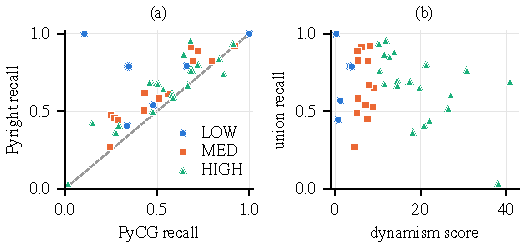
\includegraphics[width=\columnwidth]{fig_recall}
\caption{Recall against observed calls, one point per repository. (a) Pyright against PyCG; points
above the diagonal are repositories where Pyright finds more. (b) Union recall against the dynamism
score used to stratify the corpus.}\label{fig:recall}
\end{figure}

\subsection{RQ3: Static recall against runtime calls}\label{sec:rq3}

\rqThreeBody{}

\subsection{RQ4: LLMs as call resolvers}

\rqFourBody{}

% ---------------------------------------------------------------------------------------------
\section{Discussion}

\textbf{Static call graphs are less settled than their benchmarks suggest.} On micro-benchmarks
PyCG is precise; on real repositories it fails on a fifth of the corpus and its output is
seed-dependent on nearly half of the rest\ifdefined\sweepMaxDelta. The seed costs accuracy on some
repositories (PyCG's recall moved by up to \sweepMaxDelta{} across seeds), but the union with Pyright
damps it to at most \sweepUnionMaxDelta; the failures and the disagreement between analysers matter
more\fi. Tools that consume call graphs should treat each as one noisy
view, and taking the union of two analysers is cheap.

\textbf{LLMs are recall tools, not replacements.} \rqDiscussionLlm{}

\textbf{Call graphs are not reference graphs.} In a small pilot on repository-wide renames in
\texttt{click}, every rename that failed even with runtime-derived callers in context (\pilotFusedFails{} of \pilotFusedFails)
failed on a line that names the function without calling it: a dispatch-table entry, a callback
registration, a monkey-patch. No call graph, static or dynamic, holds these lines; code assistants
that retrieve context through call graphs need reference edges as well.

% ---------------------------------------------------------------------------------------------
\section{Threats to Validity}

\textbf{Ground truth is workload-conditional.} The tracer sees only what the test suites execute.
Recall is measured against the calls the tests made, a subset of the calls the program can make,
and precision only on lines that executed; a static edge that no test exercised is neither
confirmed nor counted against the tool.

\textbf{Environments.} Static extraction (RQ1, RQ2) used the frozen environments of the triage
run. The runtime traces for RQ3 and RQ4 were collected on a second x86-64 host where each
repository was installed by the same recipe rather than from the frozen dependency list, so
dependency versions may differ; the static graphs are computed from source and are unaffected. \texttt{click} and \texttt{toolz},
measured earlier, were extracted and traced on an arm64 development machine; both are pure-Python
packages, so no compiled dependency enters their graphs.

\textbf{Choice of analysers.} PyCG's repository is archived and no longer developed, but PyCG is
still the baseline in 2024--25 studies~\cite{bouzenia2024dypybench,venkatesh2025llmcg}, so its
seed dependence bears on their numbers. We did not evaluate Jarvis~\cite{huang2023jarvis}, whose
gains are reported on micro-benchmarks and a handful of applications; measuring it on the same
traces is the obvious next step.

\textbf{Tool versions and configuration.} We measure one version of each analyser. Pyright ran
without dependencies installed. PyCG's 30-minute budget is a choice; on the two timed-out repositories we probed, the fixpoint
diverged, so a larger budget would not have helped there, but we did not probe all
\nFailTimeout{}.

\textbf{LLM sample and serving.} The LLMs answered a sample of callers, enriched for hard items,
so their scores are not directly comparable to the static scores on all items; we report every
resolver on the same sample. Models served through an API may change; we record the serving
model per answer.

\textbf{Corpus.} The corpus excludes repositories that cannot be installed from their root with
\texttt{pip} or that collect no tests, which biases it against applications and monorepos. The
runtime subset favours small, pure-Python packages whose test suites need no external services.
The LOW stratum of the runtime subset is the thinnest, with \nLowRuntime{} repositories.

% ---------------------------------------------------------------------------------------------
\section{Conclusion}

On real Python repositories, the standard static call-graph generator fails on a fifth of the corpus
and its output depends on the hash seed on nearly half of the rest, and two static analysers
disagree on a third of the edges. Measured against the calls tests actually make, \rqConclusion{}
The pinned repository list, image digests,
dependency-lock hashes, extraction and tracing code, and all results will be released upon
publication, so that the numbers can be re-measured as tools change.

\section*{Acknowledgment}
LLM queries were made through the co-authors' Groq API accounts, with Groq's permission.

\bibliographystyle{IEEEtran}
\bibliography{refs}

\end{document}
